\section{电能在国民经济中的重大意义}\label{sec:10-14}

大家都知道,电能的应用非常广泛。那么,它有哪些优点呢?

首先,电能使用起来非常方便。它能够方便地转化为其他形式的能,来满足生产和生活的各种需要。
例如,它能够转化为光能,使电灯发光;转化为热能,使电炉发热;转化为机械能使电动机转动等等。
此外,利用电能的各种用电器,在管理和操纵方面比较简单。工作场所也容易保持干净。

其次,电能便于远距离输送,而且损失小。用电线就可以把电能输送到千百里之外的地方去。

第三,把自然界存在的各种形式的能转化为电能比较容易。
如燃料的化学能、水能、风能、太阳能以及原子能等都可以经过比较简便的过程转化为电能。

我国是世界上能源丰富的国家。我们的祖国不但有丰富的煤炭、石油等燃料,
可以用来建设火力发电站,而且还有许多大的河流,是兴建大型水力发电站的优越条件。
解放前,我国的电力工业是十分落后的,到全国解放的 1949 年,全国的发电量只有 43 亿度。
新中国成立以来,我国的电力工业有了巨大的发展。1959 年,全国的发电量达到 415 亿度。
1980 年,全国的发电量达到 3006 亿度。我国在发电机的制造技术上也已达到了先进水平。
这使我国能在自力更生的基础上建立越来越多的大型发电站。
正在兴建的葛洲坝水电站(图 \ref{fig:10-49})是万里长江上的第一个大型发电站。
建成后,预计每年平均发电 138 亿度,相当于 1949 年全国总发电量的三倍多。
在重视建设大型发电站的同时,我国也十分重视中小型发电站的建设。

\begin{figure}[H]%[htbp]
    \centering
    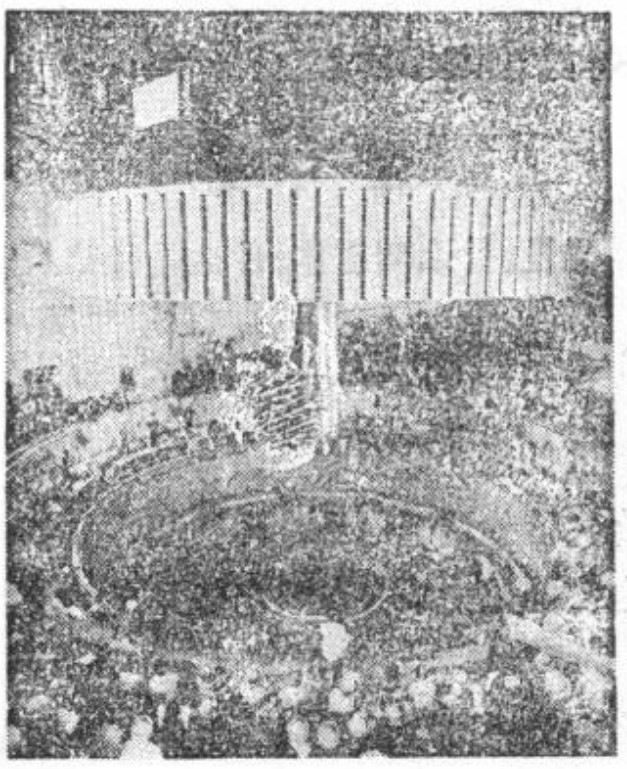
\includegraphics[width=0.7\textwidth]{../pic/czwl2-ch10-49}
    \caption{葛州坝水利枢纽工程一号机组转子吊装时的情景}\label{fig:10-49}
\end{figure}

我国的社会主义现代化建设,对电的需要量日益增加。
目前,我国除了合理地发展水力发电和火力发电外,还正在试验研究太阳能发电、风力发电、地热发电并建设原子能发电等。
总之,大力发展电力工业,对促使国民经济更快地发展,为把我国建设成为现代化的,高度文明、高度民主的社会主义国家,具有重大的意义。


\lianxi

(1) 一台发电机,输出功率是 100 千瓦, 输出电压是 250 伏特,输出电流是多少安培?

(2) 刘家峡水电站发电机组的总功率是 122.5 万千瓦,它一年(按365 天计算)能发多少度电?

